% Computer Networks homework template.
% Environment: Windows10 Home + TeXLive2019 + Visual Studio Code.
% Environment: Deepin 15.11 + TeXLive2019 + Visual Studio Code.
\documentclass[a4paper,UTF8]{article}
\usepackage{ctex}
\ctexset{
proofname = \heiti{证明}
}

\usepackage{upgreek}
\usepackage{float}

\usepackage{amsmath, amssymb, amsthm}
% amsmath: equation*, amssymb: mathbb, amsthm: proof
\usepackage{moreenum}
\usepackage{mathtools}
\usepackage{url}
\usepackage{bm}
\usepackage{enumitem}
\usepackage{graphicx}
\graphicspath{{image/}}
\usepackage{subcaption}
\usepackage{booktabs} % toprule
\usepackage[mathcal]{eucal}
\usepackage[thehwcnt = 3]{iidef}

\thecourseinstitute{中国海洋大学}
\thecoursename{计算机网络}
\theterm{2019年秋季学期}
\hwname{作业}
\slname{\heiti{解}}
\begin{document}
\courseheader
\name{姓名:秦浩 \qquad 学号:17020031051}

\begin{enumerate}

\setlength{\itemsep}{3\parskip}

\item[3-07] 要发送的数据为$1101011011$.采用$CRC$的生成多项式是$P(X) = X^4 + X + 1$.试求应添加在数据后面的余数。\\
数据在传输过程中最后一个1变成了0,问接收端能否发现?\\
若数据在传输过程中最后两个1都变成了0,问接收端能否发现?\\
采用CRC检验后,数据链路层的传输是否就变成了可靠的传输?
\begin{solution}
    \item[(1)] 由题意知,要发送的数据$M=1101011011$。除数$P=10011$,则$n=4$,由CRC检验的有关知识知,余数为$1110$;\\
    \item[(2)] 经过验证,接收端能够发现;\\
    \item[(3)] 经过验证,接收端能够发现;\\
    \item[(4)] 若仅仅采用$CRC$检验,只能做到对帧的无差错接受,并没有变成可靠的传输。  
\end{solution}

\item[3-08] 要发送的数据为$101110$.采用$CRC$的生成多项式是$P(X) = X^3 + 1$.试求应添加在数据后面的余数。
\begin{solution}
    由题意知,要发送的数据$M=101110$。除数$P=1001$,则$n=3$,由CRC检验的有关知识知,余数为$011$;
\end{solution}

\item[3-09]  一个$PPP$帧的数据部分(用十六进制写出)是7D\ 5E\ FE\ 27\ 7D\ 5D\ 7D\ 5D\ 65\ 7D\ 5E.试问真正的数据是什么(用十六进制写出)?
\begin{solution}
    真正的数据为7E\ FE\ 27\ 7D\ 7D\ 65\ 7E。
\end{solution}

\item[3-10] $PPP$协议使用同步传输技术传送比特串$0110111111111100$.试问经过零比特填充后变成怎样的比特串?若接收端收到的$PPP$帧的数据部分是$0001110111110111110110$,问删除发送端加入的零比特后变成怎样的比特串?
\begin{solution}
    经过零比特填充后变成$011011111011111000$;删除发送端加入的零比特后变成$00011101111111111110$。
\end{solution}

\item[3-16] 数据率为$10Mbit/s$的以太网在物理媒体上的码元传输速率是多少码元/秒?
\begin{solution}
    因为以太网发送的数据使用曼彻斯特编码,所以码元传输速率为$20M$码元/秒。
\end{solution}

\item[3-18] 试说明$10BASE-T$中的“$10$”、“$BASE$”和“$T$”所代表的意思。
\begin{solution}
    “10”代表$10Mbit/s$的数据率,“BASE”代表连线上的信号是基带信号,“T”代表双绞线。
\end{solution}

\item[3-20] 假定$1km$长的$CSMA/CD$网络的数据率为$1Gbit/s$。设信号在网络上的传播速率为$200000km/s$。求能够使用此协议的最短帧长。
\begin{solution}
    由题意知,信号在$1km$的网络上,单程端到端传播时延为$\frac{1}{200000}=5\upmu s$,所以争用期为$10\upmu s$,所以最短帧长为$1Gbit/s * 10\upmu s = 10000bit = 1250$字节。
\end{solution}

\item[3-21] 什么叫做比特时间?使用这种时间单位有什么好处?$100$比特时间是多少微秒?
\begin{solution}
    1比特时间就是发送1比特所需的时间,这种时间单位与数据率密切相关,为了方便可以直接使用比特作为时间单位;可以方便建立数据长度与传播时间的关系;100比特时间是$10\upmu s$。
\end{solution}

\item[3-22] 假定在使用$CSMA/CD$协议的$10Mbit/s$以太网中某个站在发送数据时检测到碰撞,执行退避算法时选择了随机数$r = 100$.试问这个站需要等待多长时间后才能再次发送数据?如果是$100Mbit/s$的以太网呢?
\begin{solution}
    $10Mbit/s$以太网争用期为$51.2\upmu s$,需要等待r个争用期,等待时间为$51.2\upmu s * 100 = 5120\upmu s$;$100Mbit/s$以太网争用期为$5.12\upmu s$,等待时间为$5.12\upmu s * 100 = 512\upmu s$;
\end{solution}

\item[3-24] 假定站点A和B在同一个$10Mb/s$以太网网段上。这两个站点之间的传播时延为$225$比特时间。现假定A开始发送一帧,并且在A发送结束之前B也发送一帧。如果A发送的是以太网所容许的最短的帧,那么A在检测到和B发生碰撞之前能否把自己的数据发送完毕?换言之,如果A在发送完毕之前并没有检测到碰撞,那么能否肯定A所发送到帧不会和B发送的帧发生碰撞?(提示:在计算时应当考虑到每一个以太网帧在发送到信道上时,在MAC帧前面还要增加若干字节的前同步码和帧定界符) 
\begin{solution}
    由题意知,A发送帧的长度为$64 + 8 = 72$字节,那么A发送完毕所需的时间为$72 * 8 = 576$比特时间。AB两个站点之间的传播时延为$225$比特时间,也就是说经过$225$比特时间B就会检测到和A发生碰撞。225比特时间之后B就不会发送数据,所以B在225比特时间之前发送数据,那么A在检测到和B发生碰撞之前不能把自己的数据发送完毕(A剩余数据发送时间大于225比特时间)。如果A在发送完毕之前并没有检测到碰撞,那么肯定A所发送到帧不会和B发送的帧发生碰撞。
\end{solution}

\item[3-25] 在上题中的站点A和B在$t=0$时同时发送了数据帧.当$t=255$比特时间,A和B同时检测到发生了碰撞,并且在$t=255+48=273$比特时间完成了干扰信号的传输.A和B在$CSMA/CD$算法中选择不同的r值退避.假定A和B选择的随机数分别是$r_A=0$和$r_B=1$.试问A和B各在什么时间开始重传其数据帧?A重传的数据帧在什么时间到达B?A重传的数据会不会和B重传的数据再次发生碰撞?B会不会在预定的重传时间停止发送数据?
\begin{solution}
    A在$t=225+48+225+96=594$比特时间开始重传数据帧,B在$t=225+48+512=785$比特时间,检验信道,若空闲,则在$t=785+96=881$比特时间发送数据;A重传的数据帧在$t=594+225=819$比特时间到达B;A重传的数据不会和B重传的数据再次发生碰撞,因为在785比特时间B检测到信道忙,所以B不会在881比特时间发送数据。
\end{solution}

\item[3-26] 以太网上只有两个站,它们同时发送数据,产生了碰撞。于是按截断二进制指数退避算法进行重传。重传次数记为$i,i=1,2,3$,试计算第1次重传失败的概率,第2次重传的概率、第3次重传失败的概率,以及一个站成功发送数据之前的平均重传次数I。 
\begin{solution}
    当$i=1$时,$r\in [0, 1]$, 重传推迟时间$[0, 2\tau]$,所以失败的概率为$\frac{1}{2}$;
    当$i=2$时,$r\in [0, 1, 2, 3]$, 重传推迟时间$[0, 2\tau, 4\tau, 6\tau]$,所以失败的概率为$\frac{1}{4}$;
    当$i=3$时,$r\in [0, 1, 2, ... , 7]$, 重传推迟时间$[0, 2\tau, ... , 14\tau]$,所以失败的概率为$\frac{1}{8}$;

    传送一次的概率为$P(1)=\frac{1}{2}$,传送两次的概率为$P(2)=\frac{1}{2}*\frac{3}{4}=\frac{3}{8}$,传送三次的概率为$P(3)=\frac{1}{2}*\frac{1}{4}*\frac{7}{8}=\frac{7}{64}$,传送四次的概率为$P(4)=\frac{1}{2}*\frac{1}{4}*\frac{1}{8}*\frac{15}{16}=\frac{15}{1024}$,所以数学期望为$I=1*\frac{1}{2}+2*\frac{3}{8}+3*\frac{7}{64}+4*\frac{15}{1024}=1.64$。
\end{solution}

\item[3-27] 有10个站连接到以太网上,试计算以下三种情况下每一个站所能得到带宽。\\
(1)10个站点连接到一个10Mbit/s以太网集线器;\\
(2)10站点连接到一个100Mbit/s以太网集线器;\\
(3)10个站点连接到一个10Mbit/s以太网交换机。
\begin{solution}
    \item[(1)] 10Mbit/s
    \item[(2)] 100Mbit/s
    \item[(3)] 10Mbit/s
\end{solution}

\item[3-28] $10Mbit/s$以太网升级到$100Mbit/s$、$1Gbit/s$和$10Gbit/s$时,都需要解决哪些技术问题?为什么以太网能够在发展的过程中淘汰掉自己的竞争对手,并使自己的应用范围从局域网一直扩展到城域网和广域网?
\begin{solution}
    $a=\frac{\tau}{T_0}$保持为很小的数值。100Mbit/s以太网可以保持最短帧长不变,电缆长度减小为原来的$\frac{1}{10}$;100Mbit/s以太网可以减小最大电缆长度或增大帧的最小长度;10Gbit/s以太网帧格式与10Mbit/s、100Mbit/s、1Gbit/s完全相同,并保留了802.3规定的以太网最小帧长和最大帧长。\\
    以太网具有可拓展、灵活、易于安装、稳健性好的优点。
\end{solution}

\item[3-30] 在图\ref{img:3-30}中,某学院的以太网交换机有三个接口分别和学院三个系的以太网相连。另外三个接口分别和电子邮件服务器、万维网服务器,以及一个连接互联网的路由器相连。图中的A,B和C都是$100Mbit/s$以太网交换机。假定所有的链路的速率都是$100Mbit/s$,并且图中的9台主机中的任何一个都可以和任何一个服务器或主机通信。试计算这9台主机和两个服务器产生的总的吞吐量的最大值,为什么? 
\begin{figure}[htbp]
    \centering
    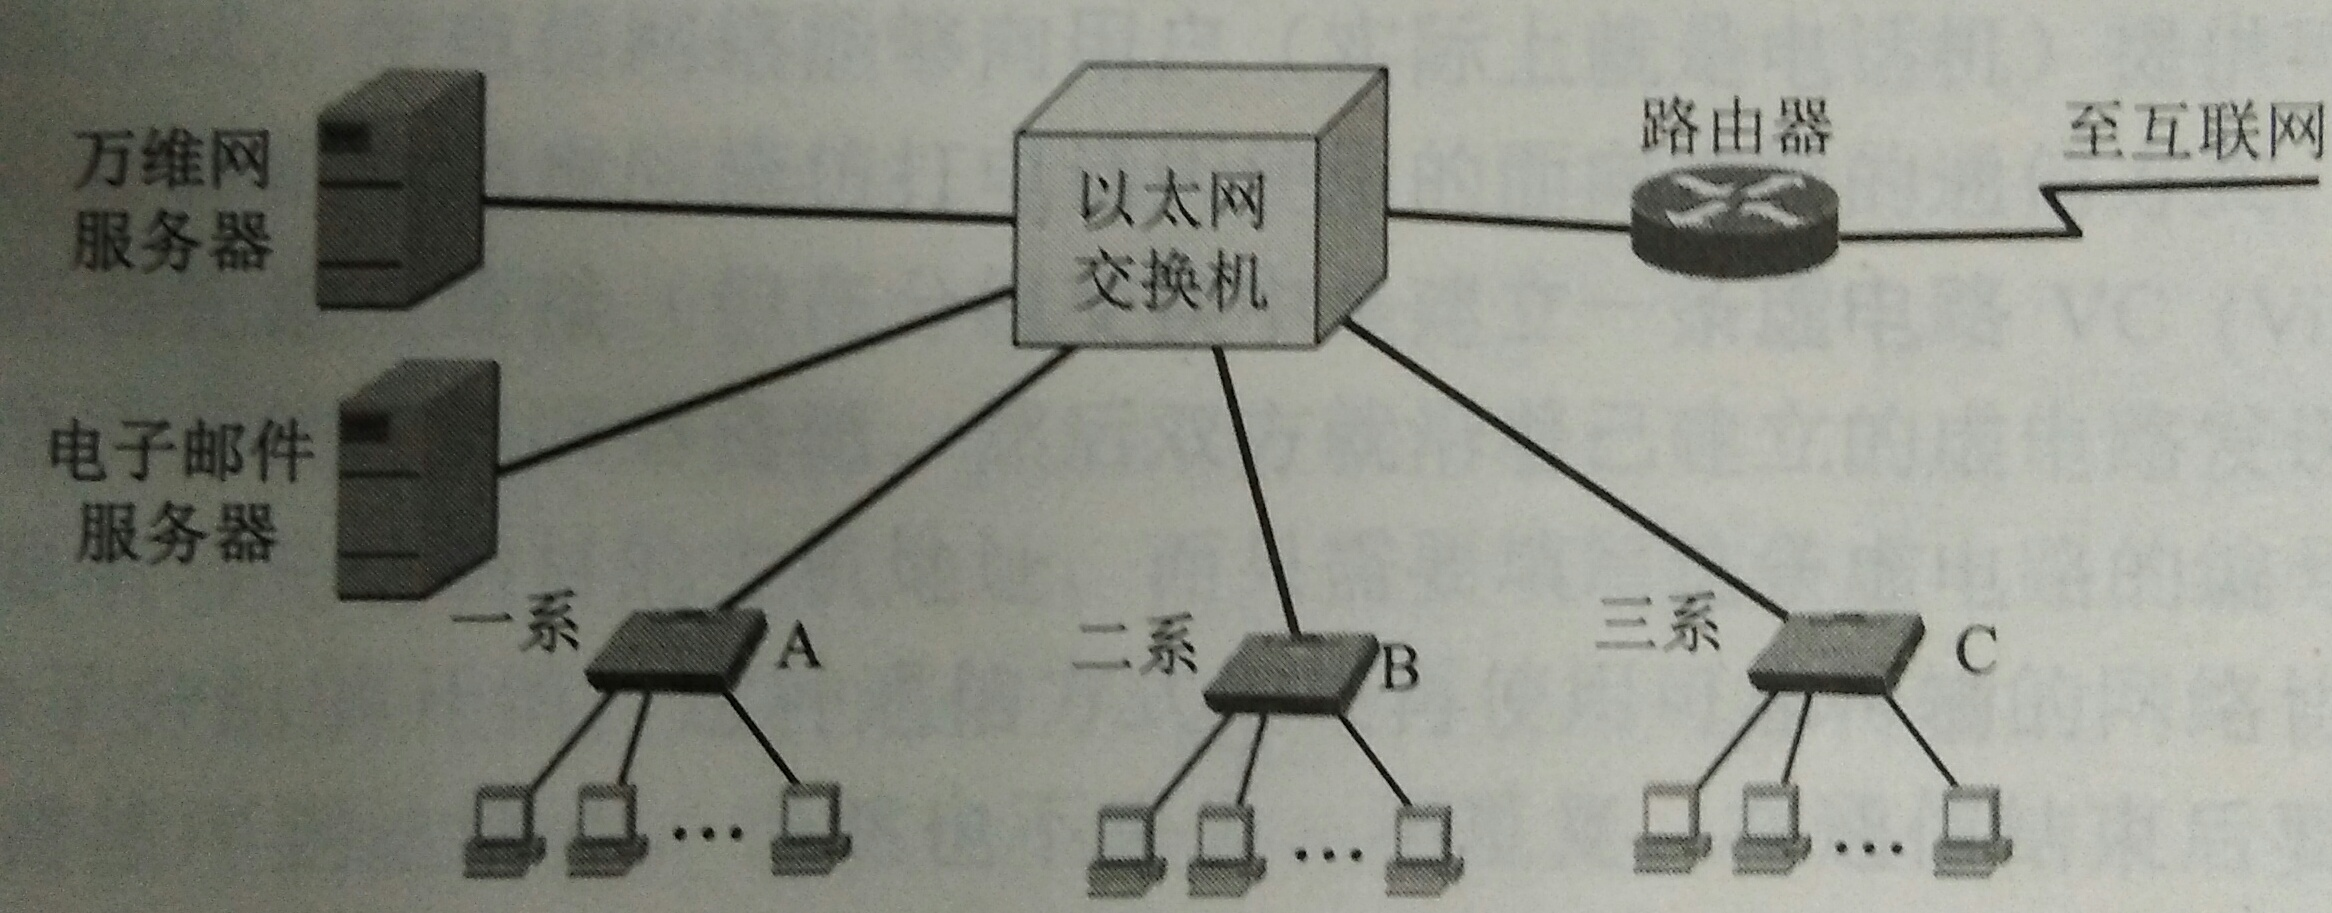
\includegraphics[scale=0.10]{3-30}
    \caption{习题3-30的图}
    \label{img:3-30}
\end{figure}
\begin{solution}
    9台主机和2个服务器都工作时的总吞吐量是$900+200=1100$Mbit/s。\\
    三个系各有一台主机分别访问两个服务器和通过路由器上网。其他主机在系内通信。
\end{solution}

\item[3-31] 假定在图\ref{img:3-30}中的所有链路的速率仍然为$100Mbit/s$,但三个系的以太网交换机都换成为$100Mbit/s$的集线器。试计算这9台主机和两个服务器产生的总的吞吐量的最大值。为什么?
\begin{solution}
    三个系的交换机换成集线器,三个系就变成了三个独立的碰撞域,所以这9台主机和两个服务器产生的总的吞吐量的最大值为$100*3+200=500$Mbit/s。
\end{solution}

\item[3-32] 假定在图\ref{img:3-30}中的所有链路的速率仍然为$100Mbit/s$,但所有的以太网交换机都换成为$100Mbit/s$的集线器。试计算这9台主机和两个服务器产生的总的吞吐量的最大值。为什么? 
\begin{solution}
    所有的以太网交换机都换成集线器,那么9台主机和两个服务器就形成一个大的碰撞域,总的吞吐量的为100Mbit/s。
\end{solution}

\item[3-33] 在图\ref{img:3-33}中,以太网交换机有6个接口,分别接到5台主机和一个路由器。在下面表的“动作”一栏中,表示先后发送了4个帧。假定在开始时,以太网交换机的交换表是空的。试把该表中其他的栏目都填写完。
\begin{figure}[htbp]
    \centering
    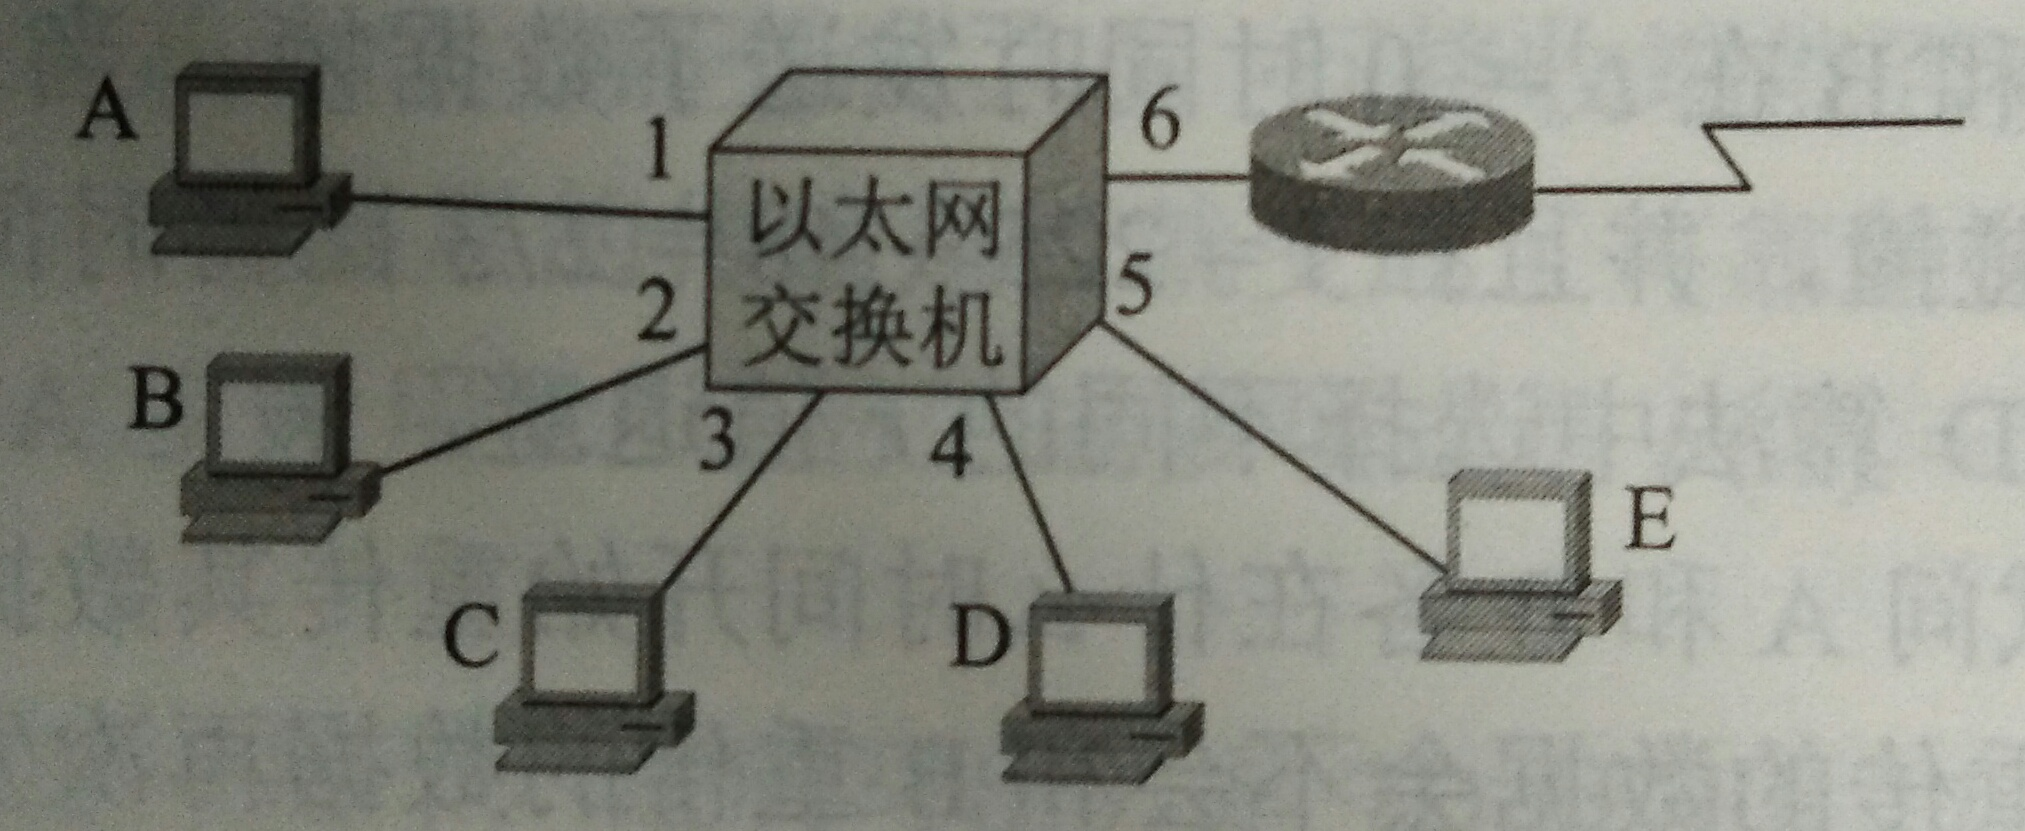
\includegraphics[scale=0.10]{3-33}
    \caption{习题3-33的图}
    \label{img:3-33}
\end{figure}
\begin{table}[H]
		\begin{tabular}{|rrrr|}
			\hline
			动作 & 交换表的状态 & 向哪些接口转发帧 & 说明 \\
			\hline
            A发送帧给D & 添加(A,1) & 2,3,4,5,6 & 开始时交换表为空,不知道D在哪个接口 \\
            \hline
			D发送帧给A & 添加(D,4) & 1 & 交换表已记录A在1接口 \\
            \hline
            E发送帧给A & 添加(E,5) & 1 & 交换表已记录A在1接口 \\
            \hline
            A发送帧给E & 不变 & 5 & 交换表已记录E在5接口 \\
			\hline
		\end{tabular}
	\end{table}
\end{enumerate}
\end{document}
\begin{equation}
\end{equation}